\subsection{Data acquisition}
The dataset used in this study is derived from the publicly available \textit{In-flight positional and energy use dataset of a DJI Matrice 100 quadcopter for small package delivery}, published by Rodrigues et al.~\cite{rodrigues2021} in \textit{Scientific Data}. This comprehensive dataset was collected over a period of seven months (April to October 2019) at an open-field test site in Penn Hills, Pennsylvania, USA (40.465690° N, 79.788281° W), under a variety of operational and environmental conditions. The data were gathered from a total of 209 autonomous flights, comprising 195 flights with active cruise phases and 14 additional hover/idle recordings, resulting in a cumulative flight duration of 10 hours and 45 minutes and a total flight distance of approximately 65 kilometers.

The experimental platform was a DJI Matrice 100 (M100) quadcopter \cite{dji2016}, a fully programmable multirotor UAV equipped with a custom sensor suite for high-resolution data acquisition. The airframe, with a total takeoff mass of 3.68 kg (unloaded), was outfitted with a payload system capable of carrying 250 g and 500 g packages, enabling the study of payload-dependent energy consumption. The vehicle was autonomously controlled via a custom Graphical User Interface (GUI) using the DJI SDK, following a predefined triangular flight path with variable cruise altitudes (25 m, 50 m, 75 m, and 100 m), ground speeds (4 m/s, 6 m/s, 8 m/s, 10 m/s, and 12 m/s), and payload masses. Each unique combination of these parameters was repeated at least three times to ensure statistical robustness and data consistency.

The dataset is publicly available under a Creative Commons Attribution 4.0 International License, and the associated codebase is released under the BSD license. This dataset provides a rare, high-fidelity, and well-documented resource for empirical modeling of UAV energy consumption, enabling validation of theoretical models and development of data-driven predictive systems such as the Random Forest model employed in this study.

\subsection{Data preparation and cleaning}
The raw flight data from the DJI~100 were reviewed and cleaned before analysis to check for errors and unrealistic values. All flight identifiers and time fields were converted into consistent formats, and a single timestamp was created from the recorded date and time. The data were then sorted chronologically for each flight and checked for duplicate records.

Physical range limits were applied to the telemetry variables based on the expected operating conditions of the DJI~100. These limits included a maximum wind speed of 60~m/s, battery voltage between 5 and 30~V, battery current within $\pm 500$~A, velocity limited to 50~m/s, total speed limited to 100~m/s, acceleration limited to 100~m/s$^2$, angular rate limited to 50~rad/s, altitude constrained between $-100$~m and 5{,}000~m, and position values restricted to a reasonable spatial bound. Orientation data were also checked to ensure that quaternion norms remained close to one. As a results, no data points were removed, indicating that the dataset was already clean and within the expected physical limits.

After cleaning the data using predefined physical limits, the measured altitude was redefined relative to the initial altitude of each flight. The relative altitude $z(t)$ in  Eq.~\eqref{eq:zt} was computed by subtracting the altitude at the start of the flight from the measured altitude at each time step.
\begin{equation}
    z(t) = \text{altitude}(t) - \text{altitude}(t=0)
    \label{eq:zt}
\end{equation}
where $ z(t) $ is the relative altitude at time $ t $.
Using this relative altitude, the vertical velocity was then derived by computing the rate of change of altitude with respect to time
using Eq.~\eqref{eq:vz} and to reduce noise in the vertical velocity signal, a one-dimensional Gaussian filter was  also applied to the vertical velocity  $v_z$  within each flight.\\
\begin{equation}
v_{z}(t) = \frac{dz(t)}{dt}
\label{eq:vz}
\end{equation}
This derived velocity was compared with the recorded vertical velocity $\texttt{velocity\_z}$ provided in the dataset. As shown in Fig.~\ref{fig:vz_diff_ways}, although both  velocities follow similar overall trends, the $\text{velocity\_z}$ exhibits larger fluctuations, while  $v_z$ is smoother, particularly during the cruise phase of flight. The observed inconsistencies also suggest a possible error in the \texttt{velocity\_z} column, which is most likely associated with the drone’s orientation rather than true vertical motion. Therefore, all further data analysis was performed using the vertical velocity derived from altitude, $v_z$.

\begin{figure}[h]
    \centering
    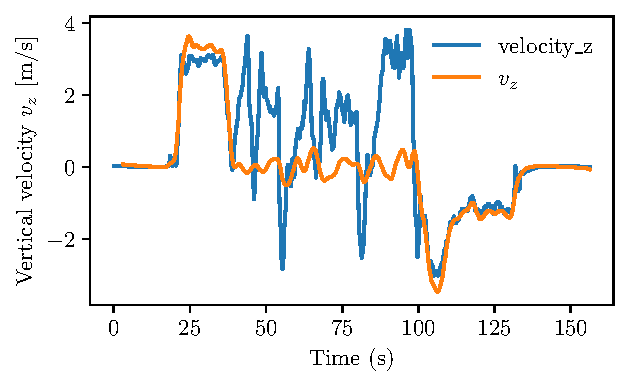
\includegraphics[width=0.9\linewidth]{figures/vz_different_ways.pdf}
    \caption{Vertical velocity versus time: comparison between given and calculated vertical velocity.}
    \label{fig:vz_diff_ways}
\end{figure}
% 
The horizontal speed $v$ was computed from the velocity components using the Euclidean norm as shown in Eq.~\eqref{eq:v}:
\begin{equation}
v = \sqrt{v_x^2 + v_y^2}  
\label{eq:v}
\end{equation}
% 
Here, $v_x$ and $v_y$ are velocities in $x$ and $y$-directions, respectively. 
Finally, the battery power was computed from voltage and current measurements as shown in Eq.~\eqref{eq:P}:
\begin{equation}
P_{\text{real}} = V_{\text{battery}} \cdot I_{\text{battery}} 
\label{eq:P}
\end{equation}
where $ P_{\text{real}} $ is the instantaneous power in watts, $ V_{\text{battery}} $ is the measured battery voltage, and $ I_{\text{battery}} $ is the measured battery current.

\subsection{Data analysis}
To better understand the aircraft’s motion prior to flight-phase classification, histograms of vertical velocity, horizontal velocity, and power were analyzed. Figure~\ref{fig:vz_hist} illustrates the histogram of the derived vertical velocity $v_z$, which displays a dominant peak near zero associated with cruise or level flight. Deviations from zero form two clear tails, indicating ascent and descent.
\begin{figure}[h]
    \centering
    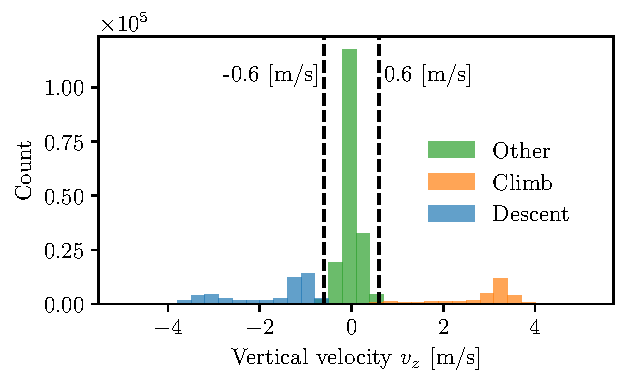
\includegraphics[width=0.9\linewidth]{figures/vertical_speed_histogram_by_phase.pdf}
    \caption{Distribution of vertical velocity as a histogram.}
    \label{fig:vz_hist}
\end{figure}
The threshold values of $\pm 0.6$~m/s were selected to define flight phases in the next section. The clear separation observed in the histogram supports different flight phase classification.

\begin{figure}[h]
    \centering
    
\includegraphics[width=0.9\linewidth]{figures/horizontal_speed_hist.pdf}
    \caption{Distribution of horizontal speed as a histogram.}
    \label{fig:v_hist}
\end{figure}
In addition to vertical motion, the horizontal speed was analyzed to further characterize the flight behavior. Figure~\ref{fig:v_hist} illustrates the histogram of the horizontal speed $v$. The distribution is strongly skewed toward low speeds, indicating that a large portion of the flight time is spent in hovering, takeoff, landing, or slow maneuvering conditions. A threshold value of $0.3$~m/s was selected to distinguish hovering from forward flight. Horizontal speeds below this threshold are classified as no forward motion. At higher speeds, the histogram exhibits multiple peaks, which correspond to different predefined forward-flight velocities. 

Finally, the power consumption was analyzed to capture the energetic characteristics of different flight conditions. Figure~\ref{fig:power_hist} shows the histogram of the measured battery power $P_{\text{real}}$, which exhibits a strong concentration at low power values corresponding to idle, hovering, or ground operation, along with a broader peak at higher power levels associated with active flight. Based on this distribution, a threshold value of 50~W was selected to distinguish between low-power and active-flight regimes. This threshold is consistent with findings by \cite{patterson2018}, who report that power during ground operations is approximately 10\% of that during cruise flight.

\begin{figure}
    \centering
    
\includegraphics[width=0.9\linewidth]{figures/power_his.pdf}
    \caption{Distribution of battery power measured as a histogram.}
    \label{fig:power_hist}
\end{figure}

